\documentclass{article}
\usepackage{graphicx} % Required for inserting images
\usepackage[italian]{babel}
\usepackage{amsmath}
\usepackage[hidelinks]{hyperref}
\usepackage{algorithm}
\usepackage{algpseudocode}

\newcommand{\arrowstar}{\overset{*}{\Rightarrow}}

\title{Automi, Calcolabilità e Complessità}
\author{Leonardo Ganzaroli}
\date{}

\begin{document}

\maketitle

\addcontentsline{toc}{section}{\protect\numberline{}Introduzione}

\tableofcontents

\newpage

\hypersetup{allcolors=black}

\section*{Introduzione}

Questi appunti sono derivanti principalmente dalle dispense del corso di \textit{Automi, Calcolabilità e Complessità} che ho svolto durante la laurea Triennale di informatica all'università "La Sapienza".

\newpage

\section{Linguaggi}

\textbf{Definizione} Un alfabeto è un insieme finito e non vuoto di elementi detti \textit{Simboli/Caratteri}.\newline

\noindent\textbf{Definizione} Dato un alfabeto $\sum$. Si dice stringa/parola di $\sum$ una sequenza finita di simboli $\in \sum$.\newline

\noindent L'insieme di tutte le possibili stringhe generate da un alfabeto $\sum$ è indicato con $\sum^*$.\newline

\noindent\textbf{Definizione} Data una stringa $x$. La sua lunghezza è data dal numero dei suoi caratteri.\newline

\noindent Nel caso la stringa sia vuota si indica con $\epsilon$.\newline

\noindent\textbf{Definizione} Data una stringa $x=x_1x_2\ldots x_n$. La sua stringa inversa è definita come  $x^R=x_n\ldots x_2x_1$.\newline

\noindent\textbf{Definizione} Concatenare 2 stringhe $x,y\in \sum^*$ vuol dire creare una nuova stringa composta dagli elementi di $x$ seguiti da quelli di $y$.\newline

\noindent\textbf{Definizione} Dato un alfabeto $\sum$. Un linguaggio di $\sum$ è un sottoinsieme di $\sum^*$.

\newpage

\subsection{Operazioni}

Essendo degli insiemi è possibile combinare i linguaggi usando le classiche operazione insiemistiche ($\cup,\cap,\ldots)$.\newline

\noindent Sono però presenti alcune operazioni aggiuntive (i linguaggi sono sullo stesso alfabeto):\newline
\begin{itemize}
    \item \textbf{Concatenazione}

$$L_1\circ L_2=\{xy\ |\ x\in L_1,\ y\in L_2\}$$

    \item \textbf{Potenza}
    
\[
L^n =
\begin{cases}
\{\epsilon\} & \text{se } n=0 \\
L\circ L^{n-1} & \text{se } n>0
\end{cases}
\]

\item \textbf{Star di Kleene}

$$L^* = \bigcup_{n\geq0}L^n$$

\item \textbf{Plus di Kleene}

$$L^+ = L\circ L^*$$\newline
    
\end{itemize}

\subsection{Hamming}

\textbf{Definizione} La distanza di Hamming tra due stringhe è il numero di caratteri per cui differiscono:

$$d_H(x,y)=|\{i\in[1,n]\ |\ x_i\neq y_i\}| \text{ con }|x|=|y|=n$$\newline

\noindent\textbf{Definizione} Dato l'alfabeto $\{0,1,\ldots,9\}$ ed $x$ una sua stringa. Il peso di Hamming di $x$ è il suo  numero di caratteri diversi da 0:

$$w_h(x)=|\{i\in[1,n]\ |\ x_i\neq 0\}| \text{ con } n=|x|$$

\newpage

\section{Linguaggi regolari}

\subsection{Automi}

\textbf{Definizione} Un automa è una macchina che segue una serie di istruzioni in modo automatico ed ha una struttura a stati.

\subsubsection{DFA}

\textbf{Definizione} Un automa a stati finiti deterministico è una quintupla $(Q,\sum,\delta,q_0,F)$ con:
\begin{itemize}
    \item $Q$ = insieme finito degli stati
    \item $\sum$ = alfabeto finito dell'automa
    \item $\delta:Q\times \sum \rightarrow Q$ = funzione di transizione degli stati
    \item $q_o\in Q$ = stato iniziale
    \item $F\subseteq Q$ = insieme degli stati accettanti\newline
\end{itemize}

\noindent La funzione di transizione si può esprimere in forma estesa $\delta^*:Q\times\sum^*\rightarrow Q$ definendola ricorsivamente come:

\[
\begin{cases}
\delta^*(q,\epsilon)=\delta(q,\epsilon)=q\\
\delta^*(q,aw)=\delta^*(\delta(q,a),w) & \text{con } a\in\sum,\ w\in\sum^* 
\end{cases}
\]\newline

\noindent Un DFA accetta una certa stringa $x=x_1x_2\ldots x_n$ se esiste una sequenza di stati $s_0s_1\ldots s_n\in Q$ tali che:
\begin{itemize}
    \item $s_0=q_0$
    \item $\forall\ i \in [0,n-1] \ \ \delta(s_i,x_{i+1})=s_{i+1}$
    \item $s_n\in F$\newline
\end{itemize}

\noindent\textbf{Definizione} Il linguaggio di un automa è l'insieme di tutte le stringhe accettate da esso, simmetricamente si dice che l'automa riconosce quel linguaggio.\newline

\newpage

\noindent\rule{\textwidth}{0.5pt}\newline

\noindent Esempio:\newline

\begin{figure}[ht]
    \centering
    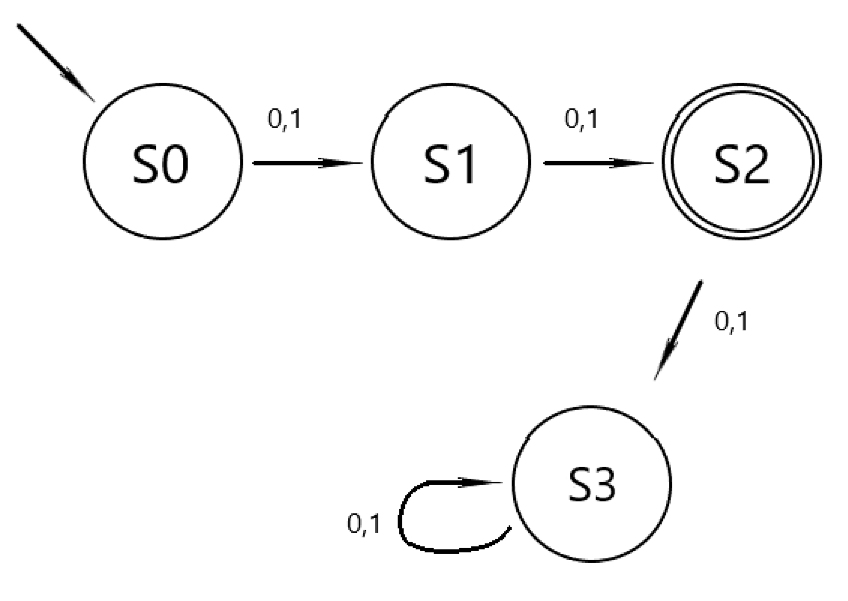
\includegraphics[width=0.7\linewidth]{DFA.png}
    \caption{Esempio DFA}
    \label{fig:dfa}
\end{figure}

\begin{itemize}
    \item $Q=\{S_0,S_1,S_2,S_3\}$
    \item $\sum = \{0,1\}$
    \item Transizioni:

        \begin{table}[ht]
            \centering
            \begin{tabular}{c|c|c}
                 & 0 & 1\\
                 \hline
                $S_0$ & $S_1$ & $S_1$\\
                \hline
                $S_1$ & $S_2$ & $S_2$\\
                \hline
                $S_2$ & $S_3$ & $S_3$\\
                \hline
                $S_3$ & $S_3$ & $S_3$\\
            \end{tabular}
            \label{tab:dfa}
        \end{table}
    
    \item $q_0=S_0$
    \item $F=\{S_2\}$
    \item $L=\{x\in \sum^*\ |\ |x|=2\}$
\end{itemize}

\noindent\rule{\textwidth}{0.5pt}\newline

\newpage

\noindent\textbf{Definizione} Una configurazione di un DFA è una coppia $(q,w)\in Q\times\sum^*$ .\newline

\noindent\textbf{Definizione} Un passo di computazione è la relazione definita come:

$$(q_i,ax)\vdash_D(q_j,x)\iff \delta(q_i,a)=q_j$$\newline

\noindent\textbf{Definizione} Una computazione è detta deterministica se ad ogni passo di computazione segue un'unica configurazione:

$$\forall \ (q,aw)\ \ \exists!\ (p,w) \ |\ (q,aw)\vdash_D(p,w)$$\newline

\subsubsection{NFA}

\noindent\textbf{Definizione} $\sum_\epsilon=\sum\ \cup\ \{\epsilon\}$\newline

\noindent\textbf{Definizione} Un automa a stati finiti non deterministico è una quintupla come un DFA, ma la sua funzione di transizione differisce:

$$\delta:Q\times\text{${\sum}_\epsilon$}\rightarrow P(Q)$$

\noindent Quindi una transizione potrebbe portare ad un qualsiasi numero di stati.\newline

\noindent Computazione:
\begin{itemize}
    \item Quando si presenta una transizione che porta in più stati la macchina crea delle copie di se stessa pari al numero di stati, ogni copia seguirà 1 dei percorsi. Si creano così dei rami di computazione che vengono eseguiti in parallelo

    \item Se non è possibile eseguire nessuna transizione con il prossimo simbolo il ramo si interrompe

    \item L'automa accetta la stringa se almeno un ramo finisce in uno stato di accettazione

    \item Se si raggiunge uno stato che ha una transizione con valore $\epsilon$ la macchina crea delle copie che seguono quegli archi ed una che resta nello stato appena raggiunto\newline
    
\end{itemize}

\newpage

\noindent\rule{\textwidth}{0.5pt}\newline

\noindent Esempio:\newline

\begin{figure}[ht]
    \centering
    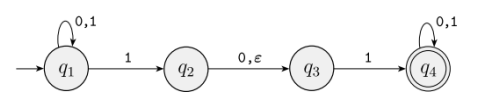
\includegraphics[width=0.65\linewidth]{NFA1.png}
    \label{fig:nfa}
\end{figure}

\noindent La computazione di questo NFA della stringa $010110$ sarà:

\begin{figure}[ht]
    \centering
    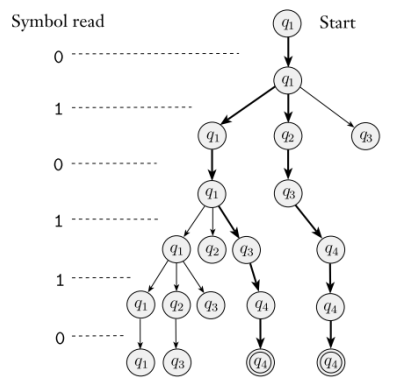
\includegraphics[width=0.6\linewidth]{NFA2.png}
    \label{fig:nfa2}
\end{figure}

\noindent\rule{\textwidth}{0.5pt}\newline

\paragraph{Equivalenza con DFA} $\ $\newline

\noindent\textbf{Definizione} Due automi si dicono equivalenti se e solo se riconoscono lo stesso linguaggio.\newline

\noindent Si nota facilmente che un NFA è una generalizzazione di un DFA, inoltre è possibile costruire un DFA equivalente di un NFA con questi passaggi:
\begin{enumerate}
    \item $Q_{DFA}=P(Q_{NFA})$
    \item Trovo $q_o$
    \item Trovo gli stati accettanti
    \item "Traduco" le transizioni
\end{enumerate}

\noindent\rule{\textwidth}{0.5pt}\newline

\noindent Esempio:\newline

\begin{figure}[ht]
    \centering
    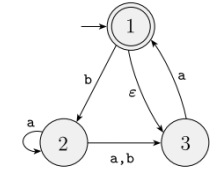
\includegraphics[width=0.4\linewidth]{trans.png}
    
    \vspace{30pt}
    
    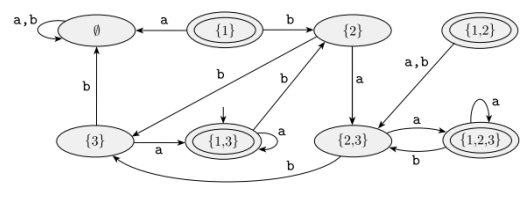
\includegraphics[width=\linewidth]{trans2.png}
    \label{fig:nfa_to_dfa}
    \caption{Trasformazione da NFA a DFA}
\end{figure}

\noindent\rule{\textwidth}{0.5pt}\newline

\noindent\textbf{Definizione} Un linguaggio si dice regolare se e solo se esiste un DFA che lo riconosce.\newline

\noindent L'insieme dei linguaggi regolari è quindi l'insieme:

$$\text{REG}=\{L\subseteq \text{${\sum}^*$}\ |\ \exists\ \text{DFA }|\ L(\text{DFA})=L\}$$

\noindent\textit{Vista la loro equivalenza si può anche riscrivere con NFA.}

\newpage

\subsection{Espressioni regolari}

\textbf{Definizione} Dato un alfabeto $\sum$. Un espressione regolare è una stringa generata da quell'alfabeto che permette di descrivere un intero linguaggio.\newline

\noindent Si possono utilizzare le operazioni $\cup,*,\circ$ (quest'ultimo spesso omesso) per combinare tra loro le espressioni regolari.

\noindent\rule{\textwidth}{0.5pt}\newline

\noindent Alcuni esempi dato $\sum=\{0,1\}$:
\begin{itemize}
    \item $0^*10^* \rightarrow$ tutte le stringhe con un solo 1

    \item $\emptyset\rightarrow \ \{\epsilon\}$ 

    \item $\sum^*\rightarrow $ tutte le stringhe possibili

    \item $((0\sum^* 0)\cup(1\sum^* 1)\cup0\cup1)\rightarrow$ tutte le stringhe che iniziano e finiscono con lo stesso carattere

    \item  $((0\cup\epsilon)(1\cup\epsilon))\rightarrow\ \{\epsilon,0,1,01\}$
    
\end{itemize}

\noindent\rule{\textwidth}{0.5pt}\newline

\noindent Partendo dai singoli elementi e procedendo a ritroso è possibile trasformare un'espressione regolare in un NFA.

\subsubsection{GNFA}

\textbf{Definizione} Un automa a stati finiti non deterministico generalizzato è una versione alternativa di un NFA in cui sugli archi sono presenti espressioni regolari invece di singoli caratteri, in questo caso l'input viene gestito "a blocchi".\newline

\noindent La funzione di transizione diventa: 
$$\delta:(Q-\{q_{accept}\})\times(Q-\{q_{start}\})\rightarrow \text{re}(\sum)$$\newline

\noindent Inoltre è presente un unico stato accettante.\newline

\newpage

\noindent Si può trasformare un DFA in un GNFA seguendo questi passaggi:
\begin{enumerate}
    \item Aggiungere un nuovo stato iniziale con un arco $\epsilon$ uscente verso il vecchio stato iniziale
    \item Aggiungere un nuovo stato accettante con un arco $\epsilon$ entrante da ogni vecchio stato accettante
    \item Sostituire gli archi con caratteri multipli con un unico arco avente l'unione dei caratteri
    \item Aggiungere archi $\emptyset$ tra gli stati non collegati, tranne:
    \begin{itemize}
        \item tra accettante e se stesso
        \item tra ogni stato e quello iniziale
    \end{itemize}
\end{enumerate}

\noindent\rule{\textwidth}{0.5pt}\newline

\noindent Esempio:

\begin{figure}[ht]
    \centering
    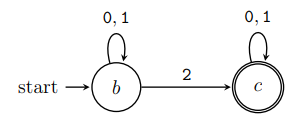
\includegraphics[width=0.5\linewidth]{GNFA.png}
    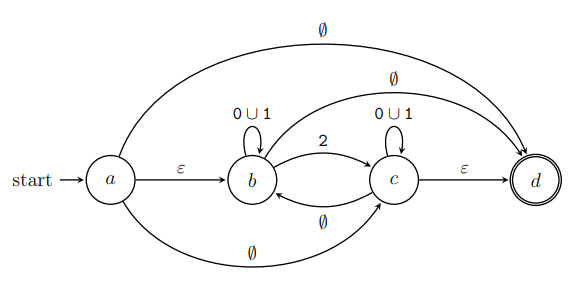
\includegraphics[width=\linewidth]{GNFA2.png}
    \caption{Trasformazione DFA in GNFA}
    \label{fig:gnfa}
\end{figure}

\noindent\rule{\textwidth}{0.5pt}\newline

\newpage

\noindent Si può trasformare un GNFA in un'unica espressione regolare seguendo l'algoritmo:\newline

\begin{algorithm}[ht]
\caption{Da GNFA a espressione regolare}
\begin{algorithmic}
\State \Comment {Dato G=GNFA}
\If {$|Q|==2$}
    \State \textbf{return} $\delta(q_{start},q_{end})$
\Else 
    \State $Q'=Q-\{q\in Q/\{q_{start},q_{accept}\}\}$
    \For {$q_i\in Q'/\{q_{accept}\}$}
        \For {$q_j\in Q'/\{q_{start}\}$}
            \State $\delta'(q_i,q_j)=\delta(q_i,q)\delta(q,q)^*\delta(q,q_j)\cup\delta(q_i,q_j)$
        \EndFor
    \EndFor
    \State $G'=(Q',\sum,\delta',q_{start},q_{accept})$
    \State \textbf{return} questa\_funzione($G'$)
\EndIf
\end{algorithmic}
\end{algorithm}

\noindent Dato che tutti gli automi visti finora e le espressioni regolari sono intercambiabili si può affermare che:

$$REG=L(DFA)=L(NFA)=L(GNFA)=L(REX)$$\newline

\subsection{Chiusura di REG}

I linguaggi regolari risultano chiusi rispetto alle principali operazioni insiemistiche viste fin'ora, ossia il nuovo insieme che si ottiene applicandole è a sua volta in REG.\newline

\noindent Si può verificare direttamente con gli automi (dati 2 linguaggi $A$ e $B$):
\begin{itemize}
    \item \textbf{Unione} $A\cup B$

    L'automa si forma inserendo un nuovo stato iniziale che ha 2 archi $\epsilon$ uscenti verso gli stati iniziali di $A$ e $B$

    \item \textbf{Intersezione} $A\cap B$

    L'automa avrà le seguenti proprietà:
    \begin{itemize}
        \item $Q=Q_A\times Q_B$
        \item $\forall\ (r_1,r_2)\in Q,\ a\in \sum \ \ \delta((r_1,r_2),a)=(\delta_A(r_1,a),\delta_B(r_2,a))$
        \item $q_0=(q_{0A},q_{0B})$
        \item $F=F_A\times F_B$
    \end{itemize}

    \item \textbf{Concatenazione} $A\circ B$

    L'automa si forma aggiungendo ad ogni stato accettante di $A$ un arco $\epsilon$ puntante allo stato iniziale di $B$

    \item \textbf{Potenza} $A^n$

    Per induzione:
    
    \begin{enumerate}
        \item $A^0$ è regolare
        \item Considerando $A^n$ regolare ho $A^{n+1}=A^n\circ A$
        \item $A^n$ e $A$ sono regolari e come visto prima la concatenazione crea un linguaggio regolare
    \end{enumerate}

    \item \textbf{Star} $A^*$

    Aggiungo un nuovo stato iniziale con arco $\epsilon$ puntante al vecchio stato iniziale ed aggiungo ulteriori archi $\epsilon$ dagli stati accettanti al vecchio stato iniziale

    \item \textbf{Complemento} $\bar{A}$

    Creo un automa con $F=Q-F_{old}$
    
\end{itemize}

\subsection{Pumping lemma}

\textbf{Definizione} Un linguaggio si dice non regolare se non esiste un DFA che lo riconosce.\newline

\noindent\textbf{Definizione} Dato $A\in$ REG. Esiste $p\in\mathbf{N}$ detto lunghezza di pumping tale che $\forall\ s \in A \text{ con } |s|\geq p\ \ \exists x,y,z\ |\ s=xyz$, inoltre:
\begin{itemize}
    \item $\forall\ i\geq0\ \ xy^iz\in A$
    \item $|y|>0$
    \item $|xy|\leq p$
\end{itemize}

\noindent\rule{\textwidth}{0.5pt}\newline

\noindent Dimostro che $\{0^n1^n\ |\ n\in \mathbf{N}\}$ non è regolare.\newline

\noindent Per assurdo esiste $p$ lunghezza di pumping, consideriamo la stringa $s=0^p1^p$, dividendola in $xyz$ risulta:
\begin{itemize}
    \item $xy=0000\ldots0$ dato che $|xy|\leq p$
    \item $y$ deve contenere almeno uno zero
    \item se $i=0\rightarrow xy^0z=xz$, ma essendo $|y|>0$ ci si ritrova con almeno uno 0 in meno e di conseguenza la stringa non appartiene al linguaggio
\end{itemize}

\noindent\rule{\textwidth}{0.5pt}\newline

\section{Linguaggi acontestuali}

\subsection{Grammatiche acontestuali}

\textbf{Definizione} Una grammatica è un insieme di regole di sostituzione di stringhe e puo produrre quest'ultime partendo da una variabile.\newline

\noindent\textbf{Definizione} Si definisce acontestualità la caratteristica per cui il lato SX di una grammatica è sempre composto da un solo simbolo.\newline

\noindent\textbf{Definizione} Una grammatica acontestuale (CFG) è una quadrupla $(V,\sum,R,S)$ con:
\begin{itemize}
    \item $V$ insieme finito delle variabili
    \item $\sum$ insieme finito dei terminali, risulta $(\sum \cap\ V)=\emptyset$
    \item $R$ insieme finito delle regole
    \item $S\in V$ variabile iniziale\newline
\end{itemize}

\noindent Le regole hanno la forma $A\rightarrow X$ dove:
\begin{itemize}
    \item $A\in V$
    \item $X\in(V\cup \sum_\epsilon)^*$\newline
\end{itemize}

\noindent \textbf{Definizione} Date $x,y,z$ stringhe. Se esiste la regola $A\rightarrow y$ allora $xAz$ produce $xyz$ e si indica con $xAz\Rightarrow xyz$.\newline

\noindent \textbf{Definizione} Date $x,y$ stringhe. $x$ deriva $y$ se $x=y$ oppure se $\exists x_1x_2x_3\ldots$ tali che $x\Rightarrow x_1\Rightarrow x_2\Rightarrow \ldots \Rightarrow y$ e si denota con $x\arrowstar y$.\newline

\noindent \textbf{Definizione} Una derivazione a sinistra è una per cui in ogni produzione interna ad essa si valuta la variabile più a sinistra.\newline

\noindent \textbf{Definizione} Date $x,y$ stringhe con $x\neq y$. Una grammatica è detta ambigua se una certa stringa $z$ può essere derivata a sinistra sia da $x$ che da $y$.

\newpage

\noindent \textbf{Definizione} Il linguaggio di una CFG è l'insieme delle stringhe che essa può generare:

$$L(G)=\{w\in{\sum}^*\ |\ S \arrowstar w\}$$\newline

\noindent Se consideriamo la classe dei linguaggi delle CFG (CFL) risulta:

$$REG\subset CFL$$

\noindent\rule{\textwidth}{0.5pt}\newline

\noindent Esempio:\newline

\noindent Una possibile grammatica è:
$$A\rightarrow0A1$$
$$A\rightarrow B$$
$$B\rightarrow\#$$

\noindent Essa ha:
\begin{itemize}
    \item $V=\{A,B\}$
    \item $\sum=\{0,1,\#\}$
    \item $A$ variabile iniziale\newline
\end{itemize}

\noindent Essa genera stringhe del tipo $000\ldots0\#111\ldots1$\newline

\noindent Si può esprimere graficamente il processo di creazione di una stringa tramite l'albero di derivazione:

\begin{figure}[ht]
    \centering
    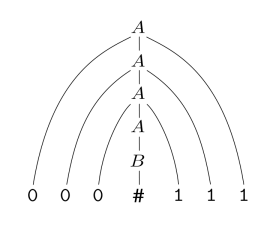
\includegraphics[width=0.4\linewidth]{der_tree.png}
    \caption{Albero di derivazione di $000\#111$}
    \label{fig:der_tree}
\end{figure}

\vspace{-10pt}

\noindent\rule{\textwidth}{0.5pt}\newline

\subsubsection{Forma normale di Chomsky}

Una CFG è in CNF se ogni sua regola è della forma:
\begin{itemize}
    \item $A\rightarrow BC$
    \item $A\rightarrow a$
    \item $S\rightarrow\epsilon$\newline
\end{itemize}

\noindent Ogni CFG si può trasformare in questa forma con questi passaggi:
\begin{enumerate}
    \item Introdurre $S_0$
    \item Eliminare le $\epsilon$-produzioni
    \item Eliminare le regole unitarie
    \item Sistemare le regole rimaste\newline
\end{enumerate}

\subsection{PDA}

\textbf{Definizione} Un automa a pila è un NFA con stack, è una sestupla $(Q,\sum,\Gamma,\delta,q_0,F)$ con:
\begin{itemize}
    \item $Q$ = insieme finito degli stati
    \item $\sum$ = alfabeto finito dell'automa
    \item $\Gamma$ = alfabeto finito della pila
    \item $\delta:Q\times {\sum}_\epsilon \times {\Gamma}_\epsilon \rightarrow P(Q\times{\Gamma}_\epsilon)$ = funzione di transizione degli stati
    \item $q_o\in Q$ = stato iniziale
    \item $F\subseteq Q$ = insieme degli stati accettanti\newline
\end{itemize}

\noindent Sugli archi si usa la notazione $a;b\rightarrow c$ in cui:
\begin{itemize}
    \item a è l'input
    \item b è il valore in cima allo stack
    \item c è il valore da inserire nello stack
\end{itemize}

\newpage

\noindent Se ho una transizione $1;b\rightarrow z$ la transizione "scatta" se:
\begin{itemize}
    \item In input c'è 1
    \item In cima alla stack c'è $b$\newline
\end{itemize}

\noindent I valori $b,c$ indicano quindi l'operazione che si va a svolgere sulla stack:
\begin{enumerate}
    \item $b\neq \epsilon$, \textbf{POP}
    \item $c\neq \epsilon$, \textbf{PUSH} di c\newline
\end{enumerate}

\noindent\rule{\textwidth}{0.5pt}\newline

\noindent Esempio:\newline

\begin{figure}[ht]
    \centering
    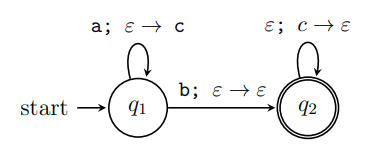
\includegraphics[width=0.5\linewidth]{PDA.png}
    \label{fig:PDA}
\end{figure}

\noindent La computazione di "aab" nel seguente PDA sarà:
\begin{enumerate}
    \item Leggi $a$, resta in $q_1$ e fai il push di c
    \item Leggi $a$, resta in $q_1$ e fai il push di c
    \item Leggi $b$, passa a $q_2$
    \item Fai il pop di $c$, resta in $q_2$
    \item Fai il pop di $c$, resta in $q_2$
\end{enumerate}

\noindent\rule{\textwidth}{0.5pt}\newline

\noindent Un PDA accetta una certa stringa $x=x_1x_2\ldots x_n$ se esiste una sequenza di stati $s_0s_1\ldots s_n\in Q$ ed una sequenza di stringhe $str_0,str_1,\ldots,str_n\in\Gamma^*$ tali che:
\begin{itemize}
    \item $s_0=q_0$
    \item $str_o=\epsilon$
    \item $\forall\ i \in [0,n-1]\ \exists a,b\in\Gamma_\epsilon ,t\in\Gamma^*\ |\ (s_{i+1},b)\in\delta(s_i,x_{i+1},a)\land str_i=at\land str_{i+1}=bt$ 
    \item $s_n\in F$\newline
\end{itemize}

\subsubsection{Equivalenza con CFG}

Si può inserire una stringa nello stack di un PDA tra 2 stati $p,q$ inserendo tra di essi degli stati intermedi in sequenza i cui archi eseguono solamente il push di un carattere alla volta. Graficamente si possono omettere inserendo sull'arco l'intera stringa.\newline

\noindent Con questa osservazione si può definire un PDA equivalente di una CFG come:

$$(\{q_0,q',q\}\cup E,\sum,V\cup\sum,\delta,q_0,\{q\})$$

\noindent Con $E$ insieme degli stati necessari per usare la notazione vista prima.\newline

\noindent Inoltre:
\begin{itemize}
    \item $\delta(q_0,\epsilon,\epsilon)=\{(q',S\$)\}$
    \item $\forall\ A\in V\ \  \delta(q',\epsilon,A)=\{(q',w)\ |\ A\rightarrow w \in R,\ w\in \Gamma^*\}$
    \item $\forall\ a\in \sum\ \ \delta(q',a,a)=\{(q',\epsilon)\}$
    \item $\delta(q',\epsilon,\$)=\{(q,\epsilon)\} $
\end{itemize}

\begin{figure}[ht]
    \centering
    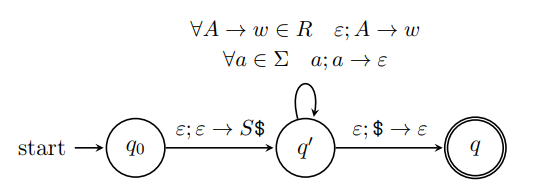
\includegraphics[width=0.7\linewidth]{CFGtoPDA.png}
    \label{fig:cfg2pda}
\end{figure}

\newpage

\noindent\rule{\textwidth}{0.5pt}\newline

\noindent Data la grammatica:

$$S\rightarrow aTb\ |\ b$$
$$T\rightarrow Ta\ |\ \epsilon$$

\begin{figure}[ht]
    \centering
    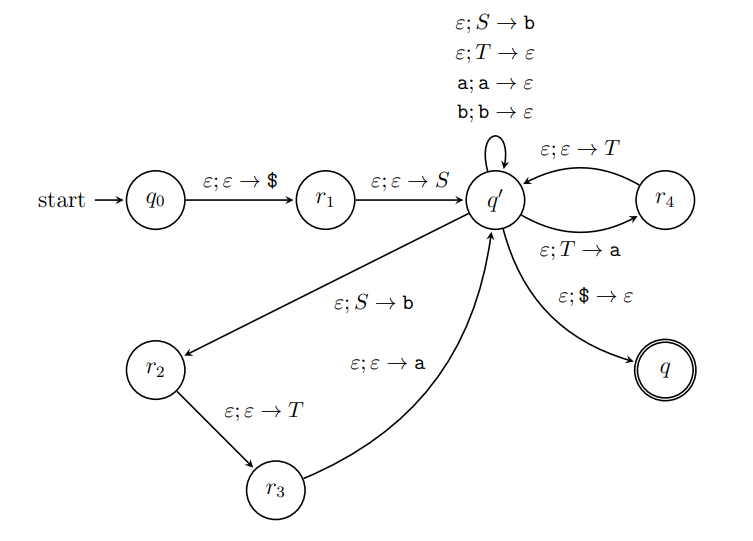
\includegraphics[width=0.8\linewidth]{CFGtoPDA_ex.png}
    \label{fig:cfg2pda_ex}
\end{figure}

\noindent\rule{\textwidth}{0.5pt}\newline

\noindent Ovviamente si può fare anche la trasformazione inversa, partendo da un PDA ne creo uno equivalente $(Q',\sum,\Gamma,\delta',q_0,\{q_{accept}\})$ tale che:
\begin{itemize}
    \item ogni transizione svolge una sola operazione, indico con $Q_\delta$ gli stati aggiunti per svolgere questa operazione
    \item $q_{accept}$ è l'unico stato accettante
    \item prima di accettare una stringa si svuota lo stack
    \item $Q'=Q\cup Q_\delta\cup \{q_{accept}\}$\newline
\end{itemize}

\noindent Creo adesso la CFG in modo che:
\begin{itemize}
    \item $V=\{A_{p,q}\ |\ p,q\in Q'\}$
    \item $S=A_{q_0,q_{accept}}$\newline
\end{itemize}

\vspace{-5pt}

\noindent Si può quindi affermare che i PDA e le CFG lavorano con la stessa classe di linguaggi (CFL).

\subsection{Chiusura CFL}

A differenza di REG i CFL sono chiusi solo rispetto ad alcune operazioni:
\begin{itemize}
    \item \textbf{Unione}

    Basta creare una grammatica equivalente partendo dalle grammatiche dei singoli linguaggi:
    \begin{itemize}
        \item Aggiungo una variabile iniziale $S$
        \item $V=(\bigcup_{i=0}^n V_i)\cup \{S\}$
        \item $\sum=\bigcup_{i=0}^n \sum_i$
        \item $R=(\bigcup_{i=0}^n R_i)\cup \{S\rightarrow S_j\ |\ j\in[1,n]\}$
    \end{itemize}
    
    \item \textbf{Concatenazione}

    Come sopra ma l'ultimo punto diventa $R=(\bigcup_{i=0}^n R_i)\cup \{S\rightarrow S_1S_2\ldots S_n\}$
    
    \item \textbf{Star}

    Creo una nuova grammatica equivalente tale che:
    \begin{itemize}
        \item Inserisco una variabile iniziale $S_0$
        \item $R'=R\cup \{S_0\rightarrow\epsilon,S_0\rightarrow S,S_0\rightarrow S_0S_0\}$
    \end{itemize}
\end{itemize}

\noindent\rule{\textwidth}{0.5pt}

\noindent Date le grammatiche:
$$G_1:A\rightarrow0A1\ |\ \epsilon$$
$$G_2:A\rightarrow1A0\ |\ \epsilon$$\newline

\noindent L'unione crea la grammatica:
$$S\rightarrow A\ |\ B$$
$$A\rightarrow0A1\ |\ \epsilon$$
$$B\rightarrow1B0\ |\ \epsilon$$

\noindent La concatenazione invece:
$$S\rightarrow AB$$
$$A\rightarrow0A1\ |\ \epsilon$$
$$B\rightarrow1B0\ |\ \epsilon$$

\noindent La star del primo:
$$S\rightarrow \epsilon\ |\ A\ |\ SS$$
$$A\rightarrow0A1\ |\ \epsilon$$

\noindent\rule{\textwidth}{0.5pt}\newline

\subsection{Pumping lemma 2.0}

\noindent\textbf{Definizione} Dato $A\in$ CFL. Esiste $p\in\mathbf{N}$ detto lunghezza di pumping tale che $\forall\ s \in A \text{ con } |s|\geq p\ \ \exists u,v,x,y,z\ |\ s=uvxyz$, inoltre:
\begin{itemize}
    \item $\forall\ i\geq0\ \ uv^ixy^iz\in A$
    \item $|vy|>0$
    \item $|vxy|\leq p$\newline
\end{itemize}

\section{Calcolabilità}

\subsection{Macchina di Turing}

Una macchina di Turing è un modello matematico computazionale che descrive una macchina astratta che manipola (legge e scrive) i dati contenuti su un nastro di lunghezza potenzialmente infinita, secondo un insieme prefissato di regole ben definite.\newline

\noindent\textbf{Definizione} Una macchina di Turing è una settupla $(Q,\sum,\Gamma,\delta,q_{start},q_{accept},q_{reject})$ con:
\begin{itemize}
    \item $Q$ = insieme finito degli stati
    \item $\sum$ = alfabeto finito della macchina
    \item $\Gamma$ = alfabeto del nastro, $\sum\subseteq\Gamma$
    \item $\sqcup$ = cella del nastro vuota, $\notin\sum,\in\Gamma$
    \item $q_{start}\in Q$ = stato iniziale
    \item $q_{accept}\in Q$ = stato accettante, se raggiunto la macchina accetta immediatamente
    \item $q_{reject}\in Q$ = stato rifutante, se raggiunto la macchina rifiuta immediatamente
    \item $\delta:(Q-\{q_{accept},q_{reject}\})\times \Gamma \rightarrow Q\times\Gamma\times\{L,R\}$ = funzione di transizione degli stati\newline
\end{itemize}

\noindent Sugli archi si usa la notazione $a;b\rightarrow X$ in cui:
\begin{itemize}
    \item $a$ è il simbolo letto sul nastro
    \item $b$ è il simbolo scritto sul nastro al posto di $a$
    \item $X$ è lo spostamento a sinistra(L) o a destra(R)\newline
\end{itemize}

\noindent\textbf{Definizione} Una stringa $uqav$ è detta configurazione di una TM se:
\begin{itemize}
    \item $q\in Q$, stato attuale
    \item $a\in \Gamma$, simbolo della cella attuale
    \item $u\in \Gamma^*$, simboli precedenti ad $a$ sul nastro
    \item $v\in \Gamma^*$, simboli successivi ad $a$ sul nastro\newline
\end{itemize}

\noindent Data una configurazione $uaq_ibv$:
\begin{itemize}
    \item essa produce $uq_jacv \iff \delta(q_i,b)=(q_j,c,L)$
    \item essa produce $uacq_jv \iff \delta(q_i,b)=(q_j,c,R)$\newline
\end{itemize}

\noindent Una TM accetta una certa stringa $x\in\sum^*$ se esiste una sequenza di configurazioni $c_1c_2\ldots c_k$ tali che:
\begin{itemize}
    \item $c_1=q_{start}w$
    \item $\forall\ i \in [1,k-1]\ \ c_i \text{ produce } c_{i+1}$ 
    \item $q_{accept}\in c_k$\newline
\end{itemize}

\noindent\rule{\textwidth}{0.5pt}\newline

\noindent Esempio:\newline

\noindent La TM che riconosce il linguaggio $\{01^n0\ |\ n\in\mathbf{N}\}$ è:\newline

\begin{figure}[ht]
    \centering
    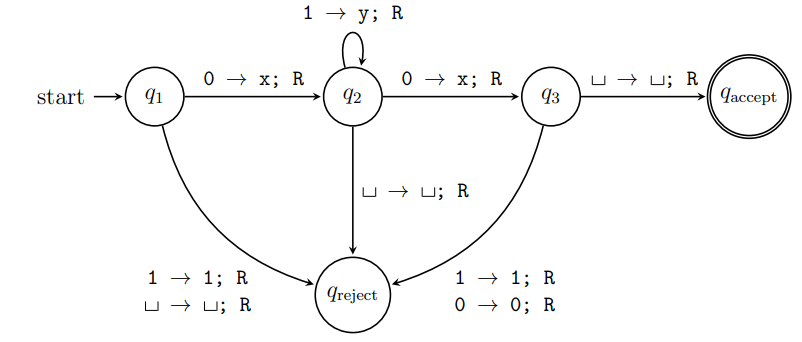
\includegraphics[width=0.85\linewidth]{TM.png}
    \label{fig:tm}
\end{figure}

\noindent\rule{\textwidth}{0.5pt}\newline

\noindent\textbf{Definizione} Una TM è detta decisore se termina sempre l'esecuzione, inoltre si dice che decide il suo linguaggio.\newline

\noindent L'insieme dei linguaggi Turing-riconoscibili è definito come:

$$\text{REC}=\{L\subseteq \text{${\sum}^*$}\ |\ \exists\ \text{TM }|\ L(\text{TM})=L\}$$\newline

\noindent Quello dei linguaggi coTuring-riconoscibili invece:

$$\text{coREC}=\{L\subseteq \text{${\sum}^*$}\ |\ \bar{L}\in REC \}$$\newline

\noindent Sostituendo la TM con un decisore ottengo invece l'insieme DEC dei linguaggi Turing-decidibili, risulta $DEC\subset REC$, inoltre $DEC=REC\cap coREC$.

\subsubsection{Varianti}
\begin{itemize}
    \item \textbf{Stay-put}

    Oltre ad andare a SX/DX può anche restare sulla cella corrente.

    \item \textbf{Multinastro}

    \item \textbf{Non deterministica}

    \item \textbf{Enumeratore}

    È connessa ad una "stampante" tramite cui stampa tutte le stringhe di un linguaggio in ordine casuale e con possibili ripetizioni, il nastro di input è vuoto.
    
\end{itemize}

\subsubsection{Tesi di Church-Turing}

Data una funzione $f$:

$$f \text{ è computabile da un algoritmo }\iff f \text{ è computabile da una TM}$$\newline

\noindent In alternativa si può dire :\textit{ Se un problema è umanamente calcolabile, allora esisterà una macchina di Turing in grado di risolverlo}.\newline

\noindent Quindi è possibile affermare che TM ed algoritmi sono equivalenti tra loro, implicando che ogni tipo di computazione si può svolgere tramite TM.\newline

\noindent\textbf{Definizione} Una TM è detta universale se può simulare qualsiasi altra TM.\newline

\noindent\textbf{Definizione} Un modello di calcolo è detto Turing-completo se è equivalente ad una TM universale.\newline

\subsection{Decidibilità}

\subsubsection{Problemi decidibili}

\textbf{Definizione} Dato un oggetto $O$. La sua codifica $\langle O\rangle$ è una stringa che ne descrive le caratteristiche.\newline

\noindent\textbf{Definizione} Il linguaggio per il problema dell'accettazione è definito come:

$$A_x=\{\langle A,w\rangle\ |\ A\text{ è } X,w\in L(A) \}$$\newline

\noindent $X$ può essere:
\begin{itemize}
    \item DFA

    Se la codifica è giusta la TM simula il DFA con input $w$ ed accetta/rifiuta in base allo stato finale della simulazione.
    
    \item NFA

    Si trasforma in un DFA equivalente e si esegue come visto sopra.
    
    \item REX

    Si trasforma in un NFA equivalente e si esegue come visto sopra.
    
    \item CFG

    Si trasforma in CNF e successivamente:
    \begin{itemize}
        \item Se $|w|=0 \text{ e } S\rightarrow \epsilon\in G_{CNF}$ allora accetta, altrimenti rifiuta

        \item Se $|w|\geq1$ genera tutte le produzioni con lunghezza $2|w|-1$ e se $w$ è tra queste accetta, rifiuta altrimenti\newline
        
    \end{itemize}
    
\end{itemize}

\newpage

\noindent\textbf{Definizione} Il linguaggio per il problema del vuoto è definito come:

$$E_x=\{\langle A\rangle\ |\ A\text{ è } X,L(A)=\emptyset \}$$\newline

\noindent $X$ può essere:
\begin{itemize}
    \item DFA

    Se la codifica è giusta la TM marca lo stato iniziale e tutti quelli che hanno archi entranti da stati marcati in modo iterativo, se alla fine uno stato accettante è marcato accetta, altrimenti rifiuta.
    
    \item CFG

    Se la codifica è giusta la TM marca i terminali e tutte le regole che hanno nella parte dx terminali o variabili marcate in modo iterativo, se alla fine S è marcato accetta, altrimenti rifiuta.\newline
    
\end{itemize}

\noindent\textbf{Definizione} Il linguaggio per il problema dell'equivalenza tra 2 DFA è definito come:

$$EQ_{DFA}=\{\langle A,B\rangle\ |\ A,B\text{ sono DFA },L(A)=L(B) \}$$\newline

\noindent Se la codifica è giusta la TM crea un DFA $C$ tale $L(C)=L(A)\bigtriangleup L(B)$, esegue poi il problema del vuoto su $C$ ed accetta/rifiuta in base al risultato di quella simulazione.\newline

\noindent Tutti i linguaggi visti in questa sezione portano inevitabilmente alla fine dell'esecuzione, quindi si considerano Turing-decidibili.

\subsubsection{Argomento diagonale di Cantor}

\textbf{Definizione} L’argomento diagonale di Cantor è una tecnica dimostrativa atta a dimostrare
l’esistenza o meno di una funzione biettiva tra due insiemi A e B disponendo
i loro elementi in forma tabellare.\newline

\noindent In particolare si può usare per provare che un certo insieme non è numerabile se non esiste una funzione biunivoca da $\mathbf{N}$ all'insieme.\newline

\newpage

\noindent\rule{\textwidth}{0.5pt}\newline

\noindent Dimostrare che l'insieme delle stringhe binarie infinite non è numerabile:
\begin{itemize}
    \item Supponiamo per assurdo che esista una funzione $f:\mathbf{N}\rightarrow B$ biunivoca
    \item Considero la stringa $x$ creata invertendo la diagonale:
    
    \begin{table}[ht]
        \centering
        \begin{tabular}{c|ccccc}
            1 & \textbf{0} & 1 & 0 & 1 & \ldots\\
            2 & 0 & \textbf{1} & 0 & 1 & \ldots\\
            3 & 1 & 1 & \textbf{1} & 0 & \ldots\\
            4 & 0 & 0 & 0 & \textbf{0} & \ldots\\
            \ldots & \ldots & \ldots & \ldots & \ldots\\
        \end{tabular}
        \label{tab:cantor}
    \end{table}
    \qquad\qquad\qquad\qquad\quad In questo caso sarà $x=1001\ldots$

    \item Data la sua costruzione si avrà che la stringa non può essere immagine di nessun numero, infatti se $f(i)=x$ si dovrà avere che l'elemento sulla diagonale ($x_{i,i}$) è diverso da se stesso

    \item Quindi la funzione non è suriettiva
    
\end{itemize}

\noindent\rule{\textwidth}{0.5pt}\newline

\noindent Si può usare questo concetto per dimostrare che esistono dei linguaggi non riconoscibili da una TM.\newline

\subsubsection{Problemi indecidibili
}

I linguaggi visti prima (accettazione,vuoto,equivalenza) sono indecidibili nel caso in cui $X$ sia una TM, lo sono anche:\newline
\begin{itemize}
    \item \textbf{Terminazione} $\{\langle M,w\rangle\ |\ M \text{ è TM e } M(w) \text{ termina}\}$
    \item \textbf{Regolarità} $\{\langle M\rangle\ |\ M \text{ è TM, } L(M) \in REG\}$
\end{itemize}

\newpage

\noindent\rule{\textwidth}{0.5pt}\newline

\noindent Esempio:\newline

\noindent Si può dimostrare che l'accettazione è indecidibile usando un ragionamento simile a quello usato per l'argomento diagonale:
\begin{itemize}
    \item Per assurdo la considero decidibile da un decisore $H$
    \item Definisco la TM $D$ che dato in input $\langle M\rangle$ esegue $H$ con input $\langle M,\langle M\rangle\rangle$ e restituisce l'opposto di quella simulazione
    \item Passando a $D$ l'input $\langle D\rangle$ risulta che se $D$ accetta $\langle D\rangle$ in $H$ allora $D$ non accetta $\langle D\rangle$ portando ad una contraddizione, infatti $D$ dà il risultato opposto di se stesso
    \item Quindi il problema non è decidibile
\end{itemize}


\noindent\rule{\textwidth}{0.5pt}

\subsubsection{Riducibilità}

\textbf{Definizione} Dati due problemi A e B. Si definisce come riduzione il metodo dimostrativo tramite
cui sapendo la soluzione di B è possibile risolvere A.\newline

\noindent\rule{\textwidth}{0.5pt}\newline

\noindent Esempio:\newline

\noindent Per provare che il problema della terminazione non è decidibile riduco quello del riconoscimento ad esso:\newline
\begin{itemize}
    \item per assurdo esiste un decisore $H$ per $HALT$
    \item costruisco una TM $D$ tale che dato l'input $\langle M,w\rangle$:
    \begin{itemize}
        \item esegue $H$ con $\langle M,w\rangle$, se rifiuta allora rifiuta
        \item altrimenti simula $M$ con $w$ ed accetta se essa accetta
    \end{itemize}
\end{itemize}

$$\text{Si ha } \langle M,w\rangle\in L(D) \iff\langle M,\ w\rangle\in L(H),w\in L(M)\iff \langle M,w\rangle\in A_{TM}$$\newline

\noindent Si nota che $L(D)=A_{TM}$, quindi teoricamente $D$ sarebbe un decisore essendo basato su $H$ ma il problema dell'accettazione non è decidibile e di conseguenza neanche quello della terminazione.\newline

\noindent\rule{\textwidth}{0.5pt}\newline

\paragraph{Tramite mappatura} $\ $\newline

\noindent\textbf{Definizione} Una funzione $f:\sum^*\rightarrow\sum^*$ è detta calcolabile se esiste una TM $F$ tale che:

$$\forall\ w\in {\sum}^*\ \ F(w) \text{ termina solo con $f(w)$ sul nastro}$$\newline

\noindent\textbf{Definizione} Dati $A,B\in \sum^*, \neq \emptyset$. Si dice che $A$ è riducibile a $B$ tramite mappatura $(A\leq_m B)$ se:

$$\exists\ f:\sum^*\rightarrow\sum^*\ |\ w\in A \iff f(w)\in B$$\newline

\noindent Si ha che se $A\leq_m B$:
\begin{itemize}
    \item $B\in DEC \Rightarrow A\in DEC$
    \item $B\in REC \Rightarrow A\in REC$
    \item $A\notin DEC \Rightarrow B\notin DEC$
    \item $A\notin REC \Rightarrow B\notin REC$\newline
\end{itemize}

\noindent\rule{\textwidth}{0.5pt}\newline

\noindent Esempio:\newline

\noindent Dimostrare che $L=\{\langle M\rangle\ |\ M \text{ è TM ed accetta stringhe di lunghezza dispari}\}$ è indecidibile.\newline

\noindent Definisco una funzione tale che $A_{TM}\leq_m L$ in questo modo:
\begin{itemize}
    \item Dato un input $\langle M,w\rangle$
    \item Costruisco una TM $M'$ tale che:
        \begin{itemize}
            \item se l'input $|x|$ è pari rifiuta
            \item altrimenti esegui $M$ su $w$ ed accetta solo se $M$ accetta
            \item dai in output $\langle M'\rangle$\newline
        \end{itemize}
\end{itemize}

\begin{itemize}
    \item se $\langle M,w\rangle\in A_{TM} \Rightarrow L(M') \text{ contiene solo le stringhe di lunghezza dispari } \Rightarrow\langle M'\rangle\in L$

    \item altrimenti $\langle M'\rangle\notin L$

\end{itemize}

\noindent\rule{\textwidth}{0.5pt}\newline

\section{Complessità}

\noindent\textbf{Definizione} Il limite superiore asintotico (O-grande) di $f(n)$ è una funzione $g(n)$ tale che:

$$\exists c,n_0\in\mathbf{N_{\geq0}}\ |\ \forall n\geq n_0\ \ f(n)\leq c*g(n)$$\newline

\noindent\textbf{Definizione} Il limite inferiore asintotico (O-piccola) di $f(n)$ è una funzione $g(n)$ tale che:

$$\forall c\in\mathbf{R_{\geq0}}\ \ \exists n_0\in\mathbf{N_{\geq0}}\ |\ \forall n\geq n_0\ \ f(n) < c*g(n)$$\newline

\noindent Date $f,g,h:\mathbf{N}\rightarrow\mathbf{R}^+$ si ha (valgono anche per $O$-grande):
\begin{itemize}
    \item $\forall\ c\in\mathbf{R}\ \ f(n)=c*o(g(n))\Rightarrow f(n)=o(g(n))$ 
    
    \item $f(n)=o(g(n))+o(h(n))\Rightarrow f(n)=o(m(n))$ con $m(n)=max(g(n),h(n))$ 
    
    \item $f(n)=o(g(n))*o(h(n))\Rightarrow f(n)=o(g(n)*h(n))$ \newline
\end{itemize}

\subsection{Temporale}

\textbf{Definizione} Dato un decisore $D$. La complessità temporale è una funzione $f:\mathbf{N}\rightarrow\mathbf{N}$ tale che $f(n)$ è il numero di passi necessari a $D$ per processare una certa stringa lunga $n$, nel caso sia non deterministico è il massimo numero di passi necessari ad ogni ramo.\newline

\subsubsection{Classi}

\noindent\textbf{Definizione} La classe dei linguaggi decidibili in tempo $O(t(n))$ è l'insieme:

$$DTIME(t(n))=\{L\in DEC\ |\ L\text{ è decidibile da una TM in tempo }O(t(n))\}$$\newline

\noindent In modo simile definisco $NTIME$, l'unica differenza è che la TM è non deterministica.

\newpage

\paragraph{P}

$$P=\bigcup_{k=0}^{+\infty}DTIME(n^k)$$\newline

\paragraph{EXP}

$$P=\bigcup_{k=1}^{+\infty}DTIME(2^{n^k})$$\newline

\paragraph{NP}

$$P=\bigcup_{k=1}^{+\infty}NTIME(n^k)$$\newline

\paragraph{NEXP}

$$P=\bigcup_{k=1}^{+\infty}NTIME(2^{n^k})$$

\paragraph{Classi complementari} $\ $\newline

\noindent\textbf{Definizione} $coP=\{A\in DEC\ |\ \bar{A}\in P\}$\newline

\noindent\textbf{Definizione} $coNP=\{A\in DEC\ |\ \bar{A}\in NP\}$\newline

\noindent\textbf{Definizione} $coEXP=\{A\in DEC\ |\ \bar{A}\in EXP\}$

\subsubsection{Riducibilità}

\textbf{Definizione} Una riduzione in tempo polinomiale ($A\leq_m^p B$) è una riduzione tra 2 linguaggi tramite mappatura in cui $f$ è calcolabile in tempo polinomiale.

\subsubsection{Classi NP-Complete}

\textbf{Definizione} NP-Hard$=\{B\subset\sum^*\ |\ \forall\ A\in NP\ \ A\leq_m^p B\}$ con $B\neq\emptyset$.\newline

\noindent\textbf{Definizione} Un linguaggio è NP-Completo se $\in(NP\cap NP\text{-Hard})$.\newline

\subsubsection{Teorema di Cook-Levin}

Questo teorema afferma che il problema della soddisfacibilità booleana è NP-Completo.

\subsection{Spaziale}

\textbf{Definizione} Dato un decisore $D$. La complessità spaziale è una funzione $f:\mathbf{N}\rightarrow\mathbf{N}$ tale che $f(n)$ è il numero di celle usate da $D$ per processare una certa stringa lunga $n$, nel caso sia non deterministico è il massimo numero di celle usate da ogni ramo.\newline

\noindent \textbf{N.B. Le celle per l'input non vengono considerate.}\newline

\subsubsection{Classi}

\noindent\textbf{Definizione} La classe dei linguaggi decidibili in spazio $O(s(n))$ è l'insieme:

$$DSPACE(s(n))=\{L\in DEC\ |\ L\text{ è decidibile da una TM in spazio }O(s(n))\}$$\newline

\noindent In modo simile definisco $NSPACE$, l'unica differenza è che la TM è non deterministica.

\paragraph{Rapporto con il tempo} $\ $\newline

\noindent Data $f(n)$ con $f(n)\geq n$ risulta:

$$DTIME(f(n))\subseteq DSPACE(f(n))$$
$$NTIME(f(n))\subseteq NSPACE(f(n))$$\newline

\noindent Inoltre se $f(n)\geq log(n)$:

$$DSPACE(f(n))\subseteq DTIME(2^{O(f(n))})$$\newline 

\subparagraph{Teorema di Savitch} $\ $\newline

Data una funzione $f(n)\geq log(n)$ si ha:

$$NSPACE(f(n))\subseteq DSPACE(f^2(n))$$\newline

\paragraph{L}

$$L=DSPACE(log(n))$$\newline

\paragraph{PSPACE}

$$PSPACE=\bigcup_{k=1}^{+\infty}DSPACE(n^k)$$\newline

\paragraph{EXPSPACE}

$$EXPSPACE=\bigcup_{k=1}^{+\infty}DSPACE(2^{n^k})$$\newline

\paragraph{NL}

$$NL=NSPACE(log(n))$$\newline

\paragraph{NPSPACE}

$$NPSPACE=\bigcup_{k=1}^{+\infty}NSPACE(n^k)$$\newline

\paragraph{NEXPSPACE}

$$NEXPSPACE=\bigcup_{k=1}^{+\infty}NSPACE(2^{n^k})$$

\paragraph{Classi complementari} $\ $\newline

\noindent\textbf{Definizione} $coL=\{A\in DEC\ |\ \bar{A}\in L\}$\newline

\noindent\textbf{Definizione} $coPSPACE=\{A\in DEC\ |\ \bar{A}\in PSPACE\}$\newline

\noindent\textbf{Definizione} $coEXPSPACE=\{A\in DEC\ |\ \bar{A}\in EXPSPACE\}$

\subsubsection{Riducibilità}

\textbf{Definizione} Una riduzione in spazio logaritmico ($A\leq_m^L B$) è una riduzione tra 2 linguaggi tramite mappatura in cui $f$ è calcolabile in spazio logaritmico.\newline

\subsubsection{Classi NL-Complete}

\textbf{Definizione} NL-Hard$=\{B\subset\sum^*\ |\ \forall\ A\in NL\ \ A\leq_m^L B\}$ con $B\neq\emptyset$.\newline

\noindent\textbf{Definizione} Un linguaggio è NL-Completo se $\in(NL\cap NL\text{-Hard})$.\newline

\subsubsection{Teorema di Immerman-Szelepcsényi}

Il teorema afferma che la classe $NL$ è chiusa rispetto al suo complemento, ossia:

$$NL=coNL$$\newline

\subsection{Teoremi di gerarchia}

\textbf{Definizione} Una funzione $f:\mathbf{N}\rightarrow\mathbf{N}$ con $f(n)\geq log(n)$ è spazio-costruibile se:

$$g:{\sum}^*\rightarrow{\sum}^*:1^n\rightarrow f(n)_2 \text{ con $f(n)_2$ codifica binaria di $f(n)$}$$\newline

\noindent si può calcolare in O(f(n)).\newline

\noindent In egual modo si può definire una funzione tempo-costruibile.\newline

\noindent Data una funzione spazio-costruibile esiste un linguaggio decidibile da una TM in spazio $O(f(n))$ ma non in spazio $o(f(n))$.\newline

\noindent Data una funzione tempo-costruibile esiste un linguaggio decidibile da una TM in tempo $O(f(n))$ ma non in tempo $o(\frac{f(n)}{log(f(n))})$.\newline

\newpage

\subsubsection{Relazioni tra le classi}

\begin{figure}[ht]
    \centering
    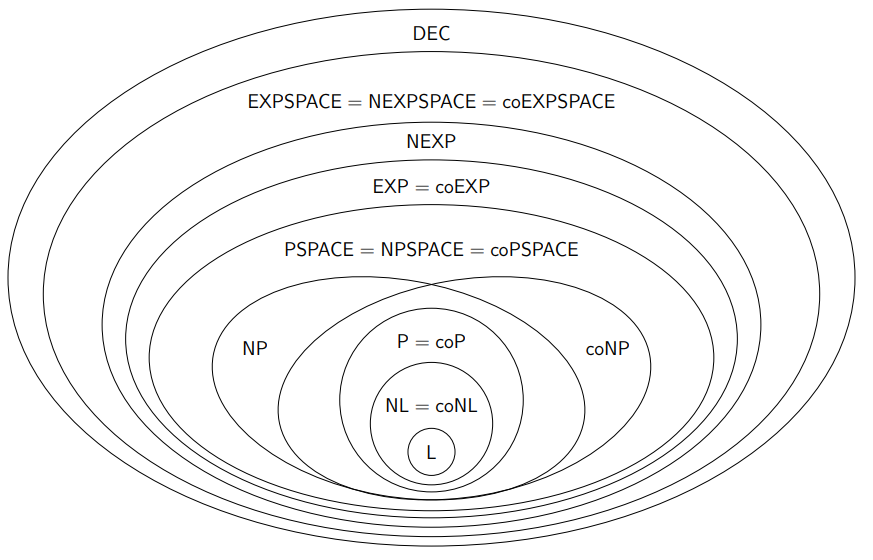
\includegraphics[width=\linewidth]{classi.png}
    \caption{Tutte le classi viste}
    \label{fig:classi}
\end{figure}

\end{document}
